\pagebreak
\subsection{Development environment}

Since the project should be developed for more than one mobile platform, it is important to make a good choice between different development environments and frameworks. The focus of this project will be on Android operating system, although application will be ported and developed for both iOS and Android.
As so, most convenient environments seem to be Eclipse and NetBeans.\newline

\begin{figure}[htb]
	\centering
	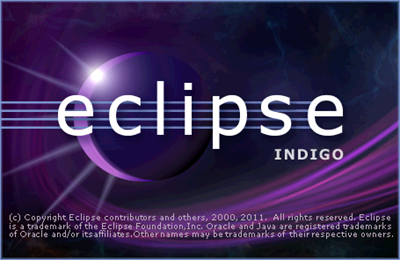
\includegraphics[width=0.3\textwidth]{organizational/development_environment/Eclipse.png}
	\caption{Eclipse Indigo}
	\label{fig:Eclipse Indigo}
\end{figure}
	
Eclipse is a multi-language software development environment comprising an integrated development environment (IDE) and an extensible plug-in system. It is written mostly in Java and can be used to develop applications in Java and, by means of various plug-ins, other programming languages, such as Android. 
To set it up and running, it is necessary to have Java Development Kit – JDK installed. Also, Android SDK must be downloaded, and with a custom plugin for the Eclipse, called Android Development Tools (ADT), integrated environment is set up to build and test Android applications.\newline

\begin{figure}[htb]
	\centering
	
\includegraphics[width=0.3\textwidth]{organizational/development_environment/netBeans.png}
	\caption{NetBeans 7.0}
	\label{fig:NetBeans}
\end{figure}

The NetBeans IDE is an open-source integrated development environment. NetBeans IDE supports development of all Java application types (Java SE including JavaFX, (Java ME, web, EJB and mobile applications) out of the box. Among other features are an Ant-based project system, Maven support, refactorings, version control (supporting CVS, Subversion, Mercurial and Clearcase).

All the functions of the IDE are provided by modules. Each module provides a well defined function, such as support for the Java language, editing, or support for the CVS versioning system, and SVN. NetBeans contains all the modules needed for Java development in a single download, allowing the user to start working immediately. Modules also allow NetBeans to be extended. New features, such as support for other programming languages, can be added by installing additional modules. For instance, Sun Studio, Sun Java Studio Enterprise, and Sun Java Studio Creator from Sun Microsystems are all based on the NetBeans IDE. It supports Android development as well, so this module is of grate importance for this project.

As already mentioned, PhoneGap will be used to develop and deploy project onto multiple platforms. Regarding all pros and cons of each development environment, for this project all team members will use Eclipse integrated with Android and PhoneGap.\newline

\begin{figure}[phonegap]
	\centering
	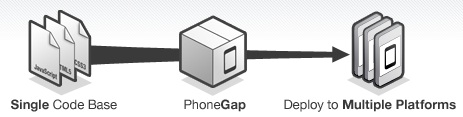
\includegraphics[width=0.8\textwidth]{organizational/development_environment/PhoneGap.jpg}
	\caption{Multiple platforms deploying}
	\label{fig:phonegap}
\end{figure}
